\documentclass{beamer}
\usepackage[ngerman]{babel}
\usepackage[utf8]{inputenc}
\usepackage{graphicx}
\usepackage{hyperref}
\usepackage{minted}
\usemintedstyle{perldoc}
\graphicspath{{./assets/}}
\setcounter{tocdepth}{1}

\title{Moderne Algorithmen für die Garbage Collection}
\subtitle{Vorstellung moderner Algorithmen für die Garbage Collection am Beispiel von Go und Java}
\date[2023]{2023}
\author{9525469, 6424019} 

\institute[DHBW Mosbach]{DHBW Mosbach}

\date{\today}

\usetheme{metropolis}
\setbeamertemplate{navigation symbols}{}
\setbeamertemplate{footline}[frame number]
\setbeamertemplate{section in toc}[sections numbered]

\begin{document}
    
    \frame{\titlepage}
    \begin{frame}
        \tableofcontents
    \end{frame}

	\section{Garbage collection}
        \begin{frame}
            \frametitle{Garbage collection}

            Garbage collection ist definiert als

            \begin{itemize}
                \item Erkennung von nicht mehr verwendeten Speicherbereichen
                \item automatisches Entfernen dieser
            \end{itemize}

            Und zielt darauf ab das obige:

            \begin{itemize}
                \item schnell
                \item effizient
                \item mit wenig Latenz
                \item mit wenig RAM und CPU Auslastung
            \end{itemize}

            umzusetzen.
        \end{frame}

        \subsection{Garbage collection - Nutzen}
            \begin{frame}
                \frametitle{Garbage collection - Nutzen}

                Befreit den Programmierer zumeist von:
                \begin{itemize}
                    \item Manueller Speicherallokierung mit \texttt{malloc}, \texttt{calloc} und \texttt{realloc}
                    \item Manueller Speicherfreigabe mit \texttt{free}
                    \item Pointer arithmetik
                \end{itemize}

                Verhindert Fehler wie: \footnote{70\% der CVE's von Chromium sind Speicherzugriffbezogen, siehe: \href{https://www.chromium.org/Home/chromium-security/memory-safety/}{https://www.chromium.org/Home/chromium-security/memory-safety/}}
                \begin{itemize}
                    \item Seg faults (illegaler Speicherzugriff) 
                    \item Use after \texttt{free} (Speicherzugriff auf bereits aufgeräumte Speicherbereiche)
                    \item Memory leaks (Speicher wird nach Verwendung nicht freigegeben)
                \end{itemize}
            \end{frame}

        \subsection{Garbage collection - Problematiken}
            \begin{frame}
                \frametitle{Garbage collection - Problematiken}
                \begin{itemize}
                    \item Peformance schlechter im Vergleich zu manuellem
                        management und borrow checker
                    \item Einfluss von GC-zyklen auf Program nicht vorhersehbar
                    \item Manuelle Allokationen mit Speicherarena effizienter
                        für große Datenmengen als jedes Objekt einzeln
                        allokieren
                \end{itemize}
            \end{frame}

    \section{Strategien}
        \begin{frame}
            \frametitle{Strategien}

            Strategien unterscheiden sich in ihrer:

            \begin{itemize}
                \item Erkennung von unerreichbaren Objekten
                \item Entfernung von unerreichbaren Objekten
                \item Latenz, RAM und CPU Verbrauch
            \end{itemize}
        \end{frame}

        \subsection{Mark \& Sweep}
            % \begin{frame}
            %     \frametitle{Strategien - Mark \& Sweep}
            %     \begin{itemize}
            %         \item Scannt den Heap anfangend von Root Objekten
            %         \item markiert Objekte die am Leben sind
            %         \item während obigem meist Stop the World
            %         \item deallokiert alle Objekte die nicht als am Leben markiert sind
            %     \end{itemize}
            % \end{frame}

            \begin{frame}
                \frametitle{Strategien - Mark \& Sweep}
                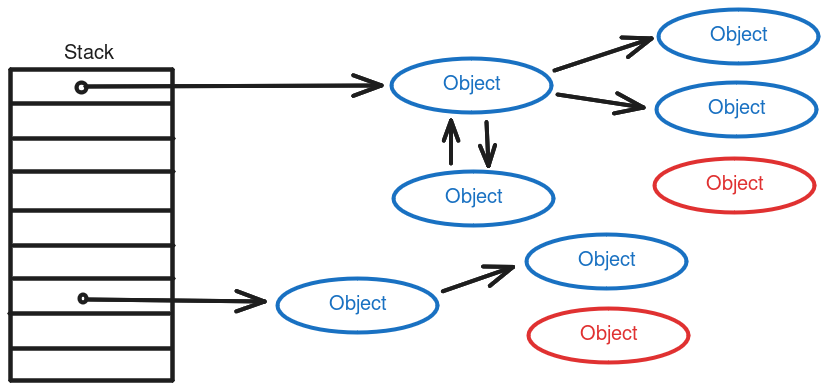
\includegraphics[width=\textwidth]{images/Mark_nd_Sweep.png}
            \end{frame}
        \subsection{Generational garbage collection}
            \begin{frame}
                \frametitle{Strategien - Generational garbage collection}
                Optimierung basierend auf der Beobachtung, dass die meisten Objekte nur kurzlebig sind (Infant Mortality)\\
                Aufteilung in drei Speicherbereiche aufgeteilt:
                \begin{itemize}
                    \item Young, bestehend aus Eden und Survivor Space
                    \item Old
                    \item Permanent
                \end{itemize}
                % Unterteilung des Heaps in die Generationen:
                % https://www.oracle.com/technetwork/tutorials/tutorials-1876574.html
                % https://www.oracle.com/webfolder/technetwork/tutorials/obe/java/G1GettingStarted/images/HeapStructure.png
                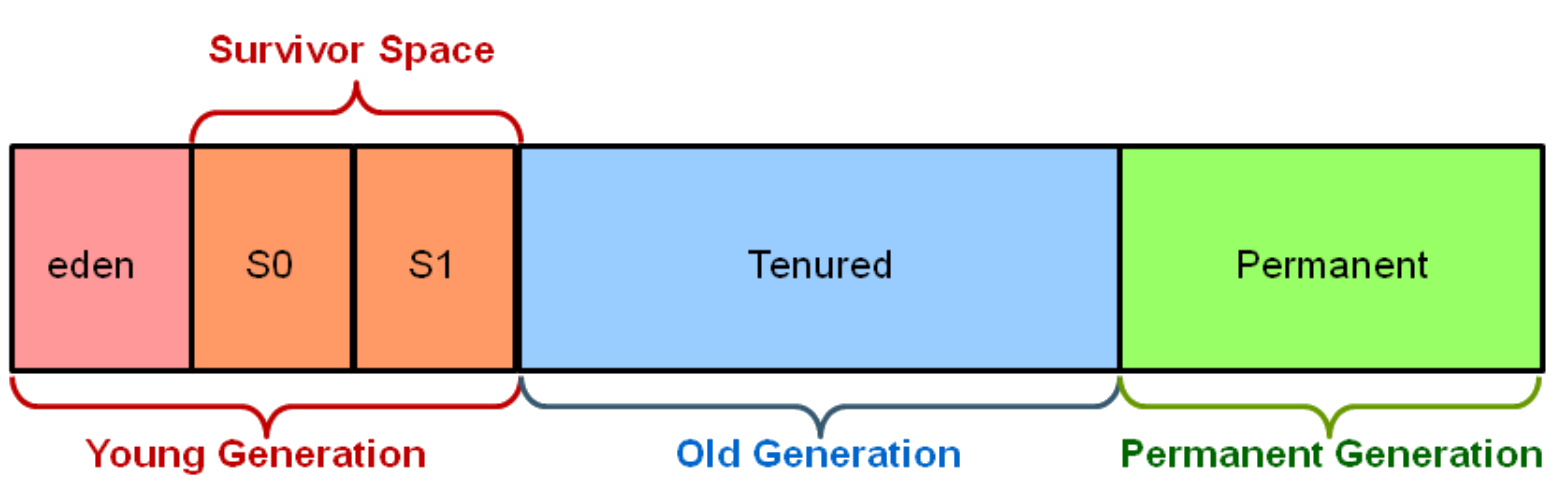
\includegraphics[width=\textwidth]{images/GenerationalGCHeapStructure.png}
            \end{frame}

            \begin{frame}
                \frametitle{Strategien - Generational garbage collection}
                \begin{itemize}
                    \item Eden
                    \begin{itemize}
                        \item Alle neuen Objekte werden hier allokiert
                        \item Objekte welche einen GC Lauf überleben, werden in den Survivor Space verschoben
                    \end{itemize}
                    \item Survivor
                    \begin{itemize}
                        \item Hier sind Objekte welche eine gewisse Zeit überlebt haben
                        \item Objekte welche eine längere Zeit überlebt haben werden in den Old Space verschoben
                    \end{itemize}
                    \item Old
                    \begin{itemize}
                        \item Hier sind Objekte welche schon länger existieren und es unwahrscheinlich ist, dass sie bald gelöscht werden
                    \end{itemize}
                \end{itemize}
                Eden wird aufgrund von Infant Mortality häufig collected, ist aber klein da lang lebende Objekte nicht dort sind.
            \end{frame}

        \subsection{Reference counting}
            \begin{frame}
                \frametitle{Strategien - Reference counting}

                \begin{itemize}
                    \item Jedes Objekt hat einen Zähler, welcher die Anzahl der Referenzen auf das Objekt zählt.\\
                    \item Beim Erstellen eines Pointers auf das Objekt wird der Zähler inkrementiert, beim Löschen dekrementiert.\\
                    \item Wird der Zähler 0, so wird das Objekt deallokiert.
                \end{itemize}
                Probleme bei Referenzzyklen: Zähler wird nie 0, Objekte werden nicht gelöscht.
            \end{frame}

            \begin{frame}[fragile]
                \frametitle{Strategien - Reference counting}

                % https://github.com/python/cpython/blob/main/Include/object.h#L214
                    \begin{minted}{c}
struct PyObject {
    // ...
    uint32_t ob_ref_local;      // local reference count
    // ...
};
                    \end{minted}

                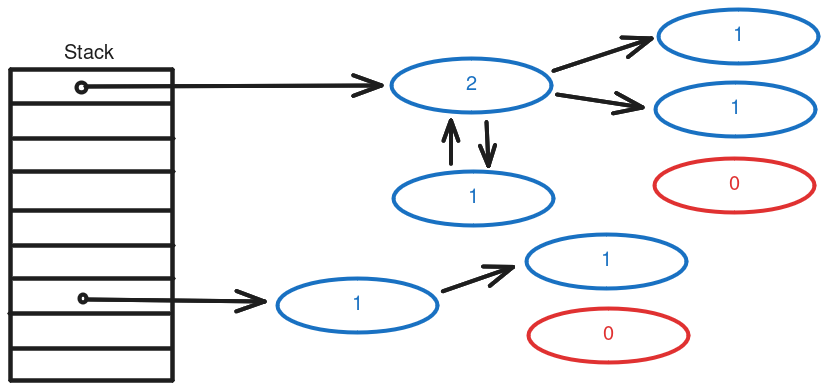
\includegraphics[width=\textwidth]{images/Reference-counting.png}
            \end{frame}


    \section{Programmiersprachen}
        \begin{frame}
            \frametitle{Programmiersprachen}

            \begin{itemize}
                \item Viele Sprachen mit und ohne GC
                \item Algorithmen, Implementierungen und Performance sehr unterschiedlich
                \item High level sprachen eher mit GC, low level eher ohne
            \end{itemize}
        \end{frame}

        \subsection{Ohne Garbage collection}
            \begin{frame}
                \frametitle{Programmiersprachen - Ohne gc}

                \begin{itemize}
                    \item C
                    \begin{itemize}
                        \item manuelles memory managment
                    \end{itemize}
                    \item C++
                    \begin{itemize}
                        \item manuelles memory managment
                        \item reference counting on demand
                    \end{itemize}
                    \item Rust
                    \begin{itemize}
                        \item borrow checker
                        \item reference counting on demand
                    \end{itemize}
                \end{itemize}
            \end{frame}

        \subsection{Mit Garbage collection}
            \begin{frame}
                \frametitle{Programmiersprachen - Mit gc}
                \begin{itemize}
                    \item Go
                    \begin{itemize}
                        \item escape analysis
                        \item mark \& sweep
                        \item Compiliert in Maschinen Code(AOT), GC in generierter Binary
                    \end{itemize}
                    \item Java
                    \begin{itemize}
                        \item mehrere garbage collectoren
                        \item generational standardmäßig
                        \item Compiliert in Bytecode(AOT), Ausführung mit Bytecode vm (JVM)
                    \end{itemize}
                    \item Python
                    \begin{itemize}
                        \item Reference counting
                        \item Erkennung von Referenzzyklen
                    \end{itemize}
                    \item JavaScript
                    \begin{itemize}
                        \item generational
                        \item JIT, Bytecode vm (V8)
                    \end{itemize}
                \end{itemize}
            \end{frame}

    \section{Implementierungen}
        \subsection{Go}
            \begin{frame}
                \frametitle{Implementierungen - Go}

                Go verwendet einen Mark \& Sweep garbage collector.

            \begin{itemize}
                    \item Concurrent
                    \item Tri-color (objekte werden eingefärbt)
                    \item Minimale Latenz durch kurzes stop the world
                        \footnote{siehe:
                        \href{https://www.youtube.com/watch?v=aiv1JOfMjm0}{https://www.youtube.com/watch?v=aiv1JOfMjm0}}
                    \item Konfigurierbar über:
                        \begin{itemize}
                            \item \texttt{GOGC}: Größe heap relativ zur Größe aller erreichbaren Objekte
                        \end{itemize}
                \end{itemize}
            \end{frame}

            \begin{frame}
                \frametitle{GO - Tri-color}

                Basierend auf Dijkstra (1978)\footnote{siehe:
                \href{https://dl.acm.org/doi/10.1145/359642.359655}{https://dl.acm.org/doi/10.1145/359642.359655}} 

                \begin{itemize}
                    \item Objekte: Weiß, Grau oder Schwarz
                    \item zu Begin des GC-Zyklus alle Objekte Weiß
                    \item GC besucht alle Roots\footnote{stack \& statische variablen, etc...} markiert als Grau
                    \item Ein Objekt wird ausgewählt und als Schwarz markiert, GC sucht ab hier nach Referenzen zu anderen Objekten
                    \item Wird ein weißes Objekt gefunden $\rightarrow$ als grau markiert.
                    \item Prozess wird wiederholt bis keine weißen Objekte mehr 
                    \item Verbleibende weiße Objekte sind nicht erreichtbar $\Rightarrow$ Deallokieren 
                \end{itemize}
            \end{frame}


        \subsection{Java}
            \begin{frame}
                \frametitle{Implementierungen - Java}

                Bei Java gibt es verschiedene GC-Implementierungen, welche via CLI Flag ausgewählt werden können.
                \begin{itemize}
                    \item Serial GC
                    \item Parallel GC
                    \item Concurrent Mark and Sweep (CMS)
                    \item Garbage First (G1) GC
                    \item Z GC
                \end{itemize}
                G1 ist Standard und wird deshalb hier vorgestellt.
            \end{frame}

            \begin{frame}
                \frametitle{Java - G1 GC Speicherstruktur}

                G1 ist ein generational GC.
                G1 allokiert Speicherblöcke, welche jeweils einer Generation zugeordnet sind.

                % https://www.oracle.com/technical-resources/articles/java/g1gc.html
                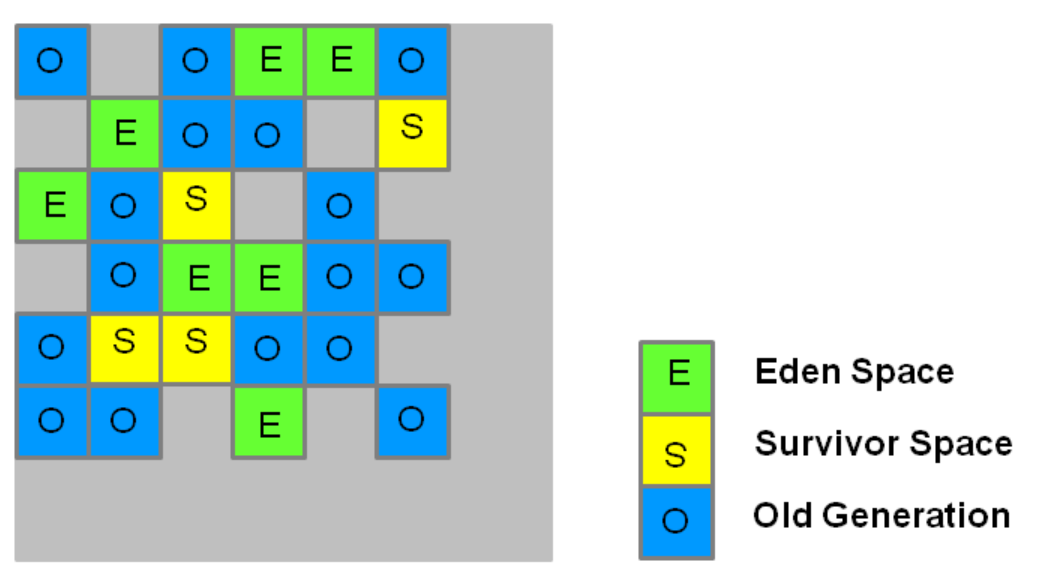
\includegraphics[width=\textwidth]{images/G1MemoryRegions.png}

            \end{frame}

            \begin{frame}
                \frametitle{Java - G1 GC Funktionsweise}

                \begin{itemize}
                    \item Wird eine Generation zu voll, so wird Garbage Collection gezielt für eine/mehrere Speicherregionen der Generation ausgeführt.
                    \item Überlebende Objekte werden in einen neuen Bereich der gleichen oder darüberliegenden Generation kopiert
                        \\$\Rightarrow$ Kompaktierung
                    \item Dannach ist die Region leer und kann neu allokiert werden.
                \end{itemize}
            \end{frame}

    \section{Performance}
        \begin{frame}
            \frametitle{Performance}

            Diverse Kriterien möglich, hier beschränkt auf:

            \begin{itemize}
                \item Speicherverbrauch: stärke RAM-Intensivität
                \item Latenz: Umfang Stoppzeiten des Programs
                \item Sicherheit: Speicherzugriffsicherheit
                \item Nutzbarkeit: Komplexität der Strategien
            \end{itemize}
        \end{frame}
        
    \section{Borrow Checking}

        \subsection{Theorie}
        \begin{frame}
            \frametitle{Borrow Checking - Theorie}

            \texttt{free} Calls können automatisch eingefügt werden, wenn der Compiler weiß wielange ein Objekt verwendet wird (\textit{Lifetime})\\
            $\Rightarrow$ automatisches Speichermanagement ohne GC\\
            Um dies möglich zu machen werden die Konzepte des \textit{Ownership} und \textit{Borrowing} eingeführt.
        \end{frame}

        \begin{frame}
            \frametitle{Borrow Checking - Ownership \& Borrowing}
            Ownership:
            \begin{itemize}
                \item Eine Variable hat einen Owner in Form einer Funktion
                \item Ownership kann von einer Funktion an eine andere übergeben werden (pass by value/return via moves)
            \end{itemize}
            Um auf Variablen an mehreren Stellen zugreifen zu können, kann diese geborrowed (verliehen) werden:
            \begin{itemize}
                \item Der Owner einer Variable kann diese an andere Strukturen verleihen.
                \item Borrowing ist nur für einen bestimmten Zeitraum möglich (Lifetime)
                \item Borrows dürfen nicht über die Lifetime des Owners hinaus bestehen, sichergestellt durch den Borrow Checker
            \end{itemize}
        \end{frame}

        \subsection{Beispiel in Rust}
        \begin{frame}[fragile]
            \frametitle{Borrow Checking - Beispiel in Rust}

            \begin{minted}{rust}
use std::io::stdin;

fn main() {
    println!("Eingabe: ");

    let line = stdin().lines().next();
    if let Some(line) = line {
        let line = line.expect("Fehler beim Lesen");
        println!("Gelesene Eingabe: \"{line}\"");
    } else {
        println!("Keine Eingabe");
    }
}
            \end{minted}
        \end{frame}

    \section{Fragen?}

\end{document}

